\documentclass[twoside,11pt,ShortChapTitles]{BYUTextbook}

\usepackage{soul}
\renewcommand{\vec}[1]{\ensuremath{\mathbf{#1}}}
\usepackage{siunitx}
\sisetup{round-mode = figures,
  round-precision = 3, scientific-notation=true}
  \usepackage{marginfix}

\usepackage{mathtools}






\setcounter{chapter}{4}

\begin{document}
\chapter{Experimental Design II: Conservation of Energy}

This week we will practice experimental design with a new context. I wont
spell out all the steps, so your lab group and you will have to work through
the experimental design steps.

Suppose you have been told that energy is conserved (I\ hope you have by now
in PH121). This is our model--the idea that energy is conserved. That is,
that it is never lost, just transferred from one form of energy to another.
A colleague suggests a method to test this model. He builds a pine-wood
derby track and a pinewood derby car.
\begin{center}
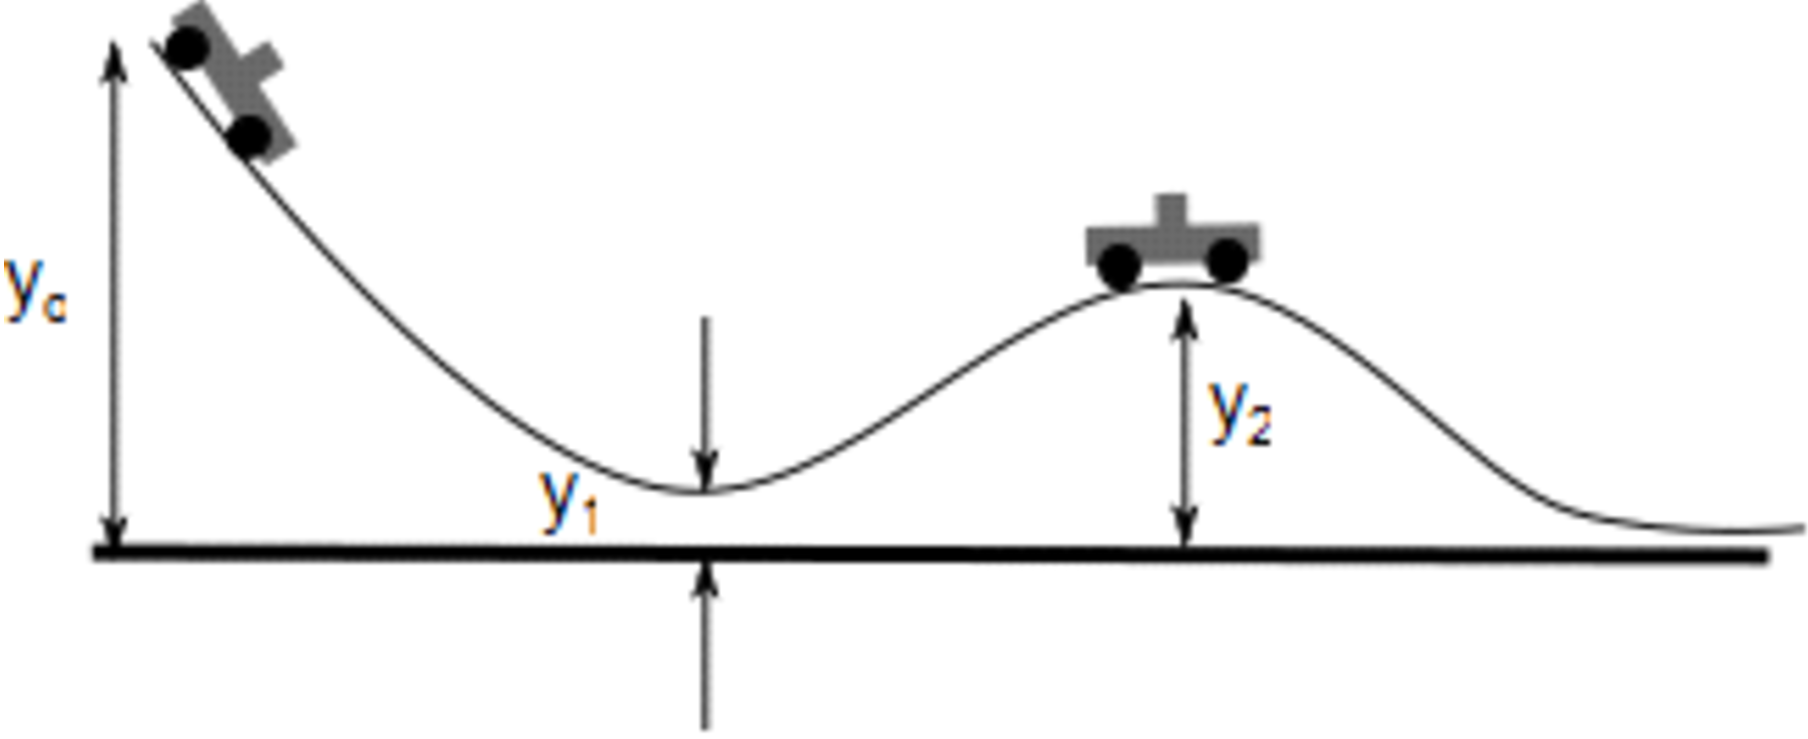
\includegraphics[width=0.5\textwidth]{Lab5_figs/LHDZMM03.png}
\end{center}
Your colleague suggests to you
that if energy is conserved, you should be able to predict the velocity of
the car at points $y_{1}$ and $y_{2}.$

Another colleague steps in and suggests that you need to be concerned about
the energy tied up in the rotational kinetic energy of the wheels. You may
not have heard about this in your PH121 class yet. She says that is OK,
because you can do a quick fix. She suggests that you should include a
factor of about 10\% of the translation kinetic energy. That is, compute the
kinetic energy in this case as%
\[
K=\left( 1.1\right) \frac{1}{2}mv^{2} 
\]%
that should account for the wheel rotational kinetic energy.

\pagebreak

\section{Assignment}

\subsection{Part 1:}

As a group design an experiment to test the model. Your design should
include the steps from lab \ref{Experimental Design} (briefly repeated here)

\begin{enumerate}
\item Identify the system to be examined. Identify the inputs and outputs.
Describe your system in your lab notebook.

\item Identify the model to be tested. Express the model in terms of an
equation representing a prediction of the measurement you will make. Record
this in your lab notebook. (If you have not solved this problem in your
PH121 class yet, call me over and we will go through it together).

\item Plan how you will know if you are successful in your experiment. Plan
graphs or other reporting devices. Record this in your lab notebook. For
today's lab, I\ will provide photogates and the car and track. If you need
other equipment, ask.

\item Rectify your equation if needed. Record this in your lab notebook.

\item Choose ranges of the variables. Record this in your lab notebook.

\item Plan the experimental procedure. Record this in your lab notebook.

\item Perform the experiment. Record this in your lab notebook. Go through
all the steps of performing an experiment. End with a conclusion that
clearly states whether your experiment supported the model, falsified the
model, or, if neither was possible, try to explain why.
\end{enumerate}

\subsection{Part 2}

Work on your proposals. They are due in two weeks. 



\end{document}